% !Mode::"TeX:UTF-8"

% -------------------- Information --------------------

\newcommand{\TITLE}{函数逼近}
\newcommand{\AUTHOR}{Jason}
\newcommand{\SUBJECT}{数值分析理论课}
\newcommand{\KEYWORDS}{}

% -------------------- Packages --------------------

\documentclass[a4paper, 12pt]{ctexart}
\usepackage{amsmath}
\usepackage{amssymb}
% \usepackage{amsthm} % 定理格式 由ntheorem代替.
\usepackage{authblk} % 作者 (见校赛论文).
\usepackage{array}
\usepackage{bigfoot} % to allow verbatim in footnote.
\usepackage{bm} % \bm for bold symbols.
\usepackage{boldline} % 长表格表格线加粗.
\usepackage{caption} % 题注.
\usepackage{commath} % abs, norm
\usepackage{enumerate}
% \usepackage{enumitem} 用enumerate包代替.
\usepackage{fancyhdr} % 脚注.
\usepackage{filecontents}
\usepackage{flafter} % 不让float出现在定义之前的地方.
\usepackage{float} % 你们这帮float给我乖乖听话 HHHHHHHHHHH.
\usepackage[T1]{fontenc} % Bera Mono Font
\usepackage{fontspec} % 字体.
\usepackage{graphicx}
\usepackage{hyperref}
\usepackage{lastpage}
\usepackage{letltxmacro} % \let
\usepackage{lipsum}
\usepackage{listings} % 排版程序语言.
\usepackage{longtable} % 长表格.
\usepackage{makecell} % 表格线加粗 \Xhline{1.2pt}.
\usepackage{mathtools} % \xleftrightarrow.
\usepackage{mathrsfs} % \mathscr
\usepackage{multirow} % 合并单元格.
\usepackage[square, numbers, sort&compress]{natbib} % 引用.
\usepackage[thmmarks, amsmath, thref]{ntheorem} % 定理格式.
\usepackage[section]{placeins} % 使图像不会显示在别的部分 若过于严格则换成[below].
\usepackage{stackrel} % 上下写 见校赛论文.
\usepackage{subcaption} % subcaption and subfigure
% \usepackage{SUBSubsubsection}
\usepackage{titlesec} % Section标题格式.
\usepackage{varioref} % For Cross References.
\usepackage[dvipsnames]{xcolor} % 颜色声明.
\usepackage{xfrac} %\sfrac{}{}
\usepackage[all, cmtip]{xy} % Commutive diagram.

% Require `ntheorem'

\usepackage[mathlines, edtable]{lineno} % Line numbers.
    %\begin{edtable}{tabular}[<args>] <entries> \end{edtable}

% Require `xcolor'

\usepackage[numbered, framed]{matlab-prettifier}
\usepackage{pgfplots}
\usepackage{tikz}

% Incompatible with `matlab-prettifier'

\usepackage[printwatermark]{xwatermark} % Foreground Watermarks.

% -------------------- Settings --------------------

% Title

\title{\TITLE}
\author{\AUTHOR}
\date{\today}

% Package: caption

\captionsetup{
    margin    =   6pt,
    font      =   small,
    labelfont =   bf
}

% Package: ctex

\setCJKfamilyfont{fzstk}{FZShuTi} % 方正舒体
\newcommand{\fzstk}{\CJKfamily{fzstk}}

% Package: fancyhdr

\setlength{\headheight}{15pt}
\lhead{Copyright \copyright\ \AUTHOR}
\rhead{Page \thepage\ of \pageref{LastPage}}

% Package: graphicx

\graphicspath{{resources/}} % 图像文件目录

% Package: hyperref

\hypersetup{
    linktoc             =   all,
    colorlinks          =   true,
    linkcolor           =   cyan,
    anchorcolor         =   black,
    citecolor           =   green,
    filecolor           =   cyan,
    menucolor           =   red,
    runcolor            =   filecolor,
    urlcolor            =   magenta,
	pdftitle           	=   {\TITLE},
	pdfauthor          	=   {\AUTHOR},
	pdfsubject         	=   {\SUBJECT},
	pdfcreator			=	{Visual Studio Code},
	pdfproducer			=	{XeLaTeX with documentclass ctexart},
	pdfkeywords        	=   {\KEYWORDS},
    bookmarksnumbered   =   true,
    pdfstartview        =   FitH,
    pdfpagelayout       =   OneColumn
}

% Package: lineno

\renewcommand{\linenumberfont}{\normalfont\scriptsize\sffamily}

\let\oldlstinputlisting\lstinputlisting
\renewcommand{\lstinputlisting}[2][\empty]{
    \par\nolinenumbers\oldlstinputlisting[#1]{#2}\linenumbers\par
}

\let\oldlstlisting\lstlisting
\let\oldendlstlisting\endlstlisting
\renewenvironment{lstlisting}
    {\par\nolinenumbers\oldlstlisting}
    {\oldendlstlisting\endnolinenumbers\par}

\let\oldtable\table
\let\oldendtable\endtable
\renewenvironment{table}
    {\par\nolinenumbers\oldtable}
    {\oldendtable\endnolinenumbers\par}

% Package: listings

%% Title

\renewcommand\lstlistingname{代码}
\renewcommand\lstlistlistingname{代码}

%% Lstinline with color box

\LetLtxMacro{\oldlstinline}{\lstinline}
\renewcommand{\lstinline}[2][]{\colorbox{lightgray}{\oldlstinline[#1]{#2}}}
\newcommand{\matlabinline}[1]{
    \lstinline[style=MATLAB-editor, basicstyle=\mlttfamily]{#1}}

\lstset{
    breaklines=true,
    backgroundcolor=\color{lightgray},
    basicstyle=\scriptsize,
    inputpath=resources/,
    numbers=left,
    numberstyle={\color{black!33}\scriptsize\sffamily},
    xleftmargin=2em,
    xrightmargin=2em
}

% Package: ntheorem

%% Theorem
\newtheorem{theorem}{Theorem}[section]
\newtheorem{lemma}[theorem]{Lemma}
\newtheorem{corollary}[theorem]{Corollary}
%% Problem
\theoremstyle{plain}
\newtheorem{problem}{Problem}[section]
%% Definition
\theoremstyle{plain}
\theoremheaderfont{\bfseries}
\theorembodyfont{\rmfamily}
\newtheorem{definition}{Definition}[section]
%% Note
\theoremstyle{plain}
\theoremheaderfont{\itshape}
\theorembodyfont{\itshape}
\newtheorem{note}{Note}[section]
%% Proof
\theoremstyle{nonumberplain}
\theoremheaderfont{\itshape}
\theorembodyfont{\upshape}
\theoremseparator{.}
\theoremsymbol{\ensuremath{\square}}
\newtheorem{proof}{Proof}
%% Solution
\theoremsymbol{\ensuremath{\blacksquare}}
\newtheorem{solution}{Solution}

% Package: pgfplot

\pgfplotsset{width=7cm, compat=1.16}

% Package: varioref

\renewcommand{\reftextbefore}
    {on the \reftextvario{preceding page}{page before}}
\renewcommand{\reftextafter}
    {on the \reftextvario{following}{next} page}
\renewcommand{\reftextfacebefore}
    {on the \reftextvario{facing}{preceding} page}
\renewcommand{\reftextfaceafter}
    {on the \reftextvario{facing}{next} page}
\renewcommand{\reftextfaraway}[1]
    {on page \pageref{#1}}

%% Label formats

\labelformat{lstlisting}{代码#1}
\labelformat{equation}{式(#1)}
\labelformat{figure}{图#1}
\labelformat{table}{表#1}

% Package: xwatermark

\newsavebox\mybox
\savebox\mybox{\tikz[color=cyan, opacity=0.2]\node{\fzstk\SUBJECT};}
\newwatermark*[
    allpages,
    angle=45,
    scale=6,
    xpos=-20,
    ypos=15
]{\usebox\mybox}

% -------------------- General new commands --------------------

\DeclareMathAlphabet{\mathsfsl}{OT1}{cmss}{m}{sl}

\DeclareMathOperator{\arcosh}{arcosh}
\DeclareMathOperator{\Arcosh}{Arcosh}
\DeclareMathOperator*{\Beta}{B}
\DeclareMathOperator*{\diff}{d}
\DeclareMathOperator{\Log}{Log}

% Expectation

\newcommand{\expect}{\operatorname{E}\expectarg}
\DeclarePairedDelimiterX{\expectarg}[1]{(}{)}{
    \ifnum\currentgrouptype=16 \else\begingroup\fi
    \activatebar#1
    \ifnum\currentgrouptype=16 \else\endgroup\fi
}

\newcommand{\innermid}{\nonscript\;\delimsize\vert\nonscript\;}
\newcommand{\activatebar}{
    \begingroup\lccode`\~=`\|
    \lowercase{\endgroup\let~}\innermid
    \mathcode`|=\string"8000
}

\newcommand{\BR}{\mathbb{R}}
\newcommand{\matr}[1]{\ensuremath{\mathsfsl{#1}}} % italic sans serif
\newcommand{\me}{\mathrm{e}}
\newcommand{\mi}{\mathrm{i}}
\newcommand{\restrict}[1]{\raisebox{-.5ex}{$\vert$}_{#1}}
\newcommand{\vect}[1]{\bm{#1}}

% -------------------- Specific new commands --------------------



% -------------------- Document --------------------

\begin{document}

    % -------------------- Title Page --------------------

    \maketitle
    \thispagestyle{empty}
    \pagenumbering{roman}

    % -------------------- Abstract Page --------------------

    % -------------------- Contents --------------------

    % \newpage
    % \tableofcontents

    % -------------------- Body --------------------

    \newpage
    \pagestyle{fancy}
    \pagenumbering{arabic}
    \linenumbers

    \begin{problem}
        试分别求函数$f(x)=\sqrt{1+x}$在区间$[0,1]$上的一次最佳一致逼近多项式
        和一次最佳平方逼近多项式.
    \end{problem}

    \begin{solution}
        因为$f''(x)=-\sfrac{3}{4}\cdot(1+x)^{-\sfrac{3}{2}}$在$[0, 1]$上不变号,
        所以可以通过几何意义求解一次最佳一致逼近多项式, 解得
        \begin{equation}
            p_{1}(x) = (\sqrt{2}-1)x+\frac{1}{8(\sqrt{2}-1)}+\frac{\sqrt{2}}{2}
        \end{equation}

        为求解最佳平方逼近多项式, 记$g(t)=\sqrt{1+\sfrac{(t+1)}{2}}$, 计算
        \begin{equation}
        \begin{aligned}
            (g, P_{0}) &= \int_{-1}^{1}{\sqrt{1+\frac{t+1}{2}}}\diff t
            \approx 2.438\\
            (g, P_{1}) &= \int_{-1}^{1}{x\sqrt{1+\frac{t+1}{2}}}\diff t
            \approx 0.137.
        \end{aligned}
        \end{equation}
        故
        \begin{equation}
        \begin{aligned}
            a_{0}^{*} &= \frac{1}{2}(g, P_{0}) \approx 1.219\\
            a_{1}^{*} &= \frac{3}{2}(g, P_{1}) \approx 0.206.
        \end{aligned}
        \end{equation}
        可知
        \begin{equation}
            q_{1}(t) \approx 1.219P_{0}(t) + 0.206P_{1}(t) = 1.219 + 0.206t.
        \end{equation}
        于是所求一次最佳平方逼近多项式即为
        \begin{equation}
            s^{*}(x) \approx 0.412t + 1.013.
        \end{equation}
    \end{solution}

    \begin{problem}
        \label{problem_squares}
        用最小二乘法, 找出形如$y=ax^{2}+b$的抛物线方程,
        使之最佳地代表\ref{table_squares}中的数据.
        
        \begin{table}[H]
            \begin{center}
                \caption{习题\ref{problem_squares}中给定的拟合数据}
                \label{table_squares}
                \begin{tabular}{cccc}
                    \Xhline{1.2pt}
                    $x$ & -1 & 0 & 1\\
                    \hline
                    $y$ & 3.1 & 0.9 & 2.9\\
                    \Xhline{1.2pt}
                \end{tabular}
            \end{center}
        \end{table}
    \end{problem}

    \begin{solution}
        建立法方程
        \begin{equation}
            \begin{pmatrix}
                3 & 2\\ 2 & 2
            \end{pmatrix}
            \begin{pmatrix}
                a \\ b
            \end{pmatrix}
            =
            \begin{pmatrix}
                6.9 \\ 6
            \end{pmatrix}
            .
        \end{equation}
        解得$a = 2.1$, $b = 0.9$. 于是所求抛物线方程为$y=2.1x^{2}+0.9$.
    \end{solution}

    \begin{problem}
        已知液体的表面张力$s$是温度$T$的线性函数$s=aT+b$,
        对某种液体有\ref{table_tension}的实验数据. 试用最小二乘法确定系数$a, b$.
        \begin{table}[H]
            \begin{center}
                \caption{表面张力--温度数据}
                \label{table_tension}
                \begin{tabular}{ccccccccc}
                    \Xhline{1.2pt}
                    $T$ & 0 & 10 & 20 & 30 & 40 & 80 & 90 & 95\\
                    \hline
                    $s$ & 68.0 & 67.1 & 66.4 & 65.6 & 64.6 & 61.8 & 61.0 & 60.0\\
                    \Xhline{1.2pt}
                \end{tabular}
            \end{center}
        \end{table}
    \end{problem}

    \begin{solution}
        输入数据后, 利用MATLAB的曲线拟合工具箱我们可以方便的得出拟合结果, 如下图.
        \begin{figure}[H]
            \centering
            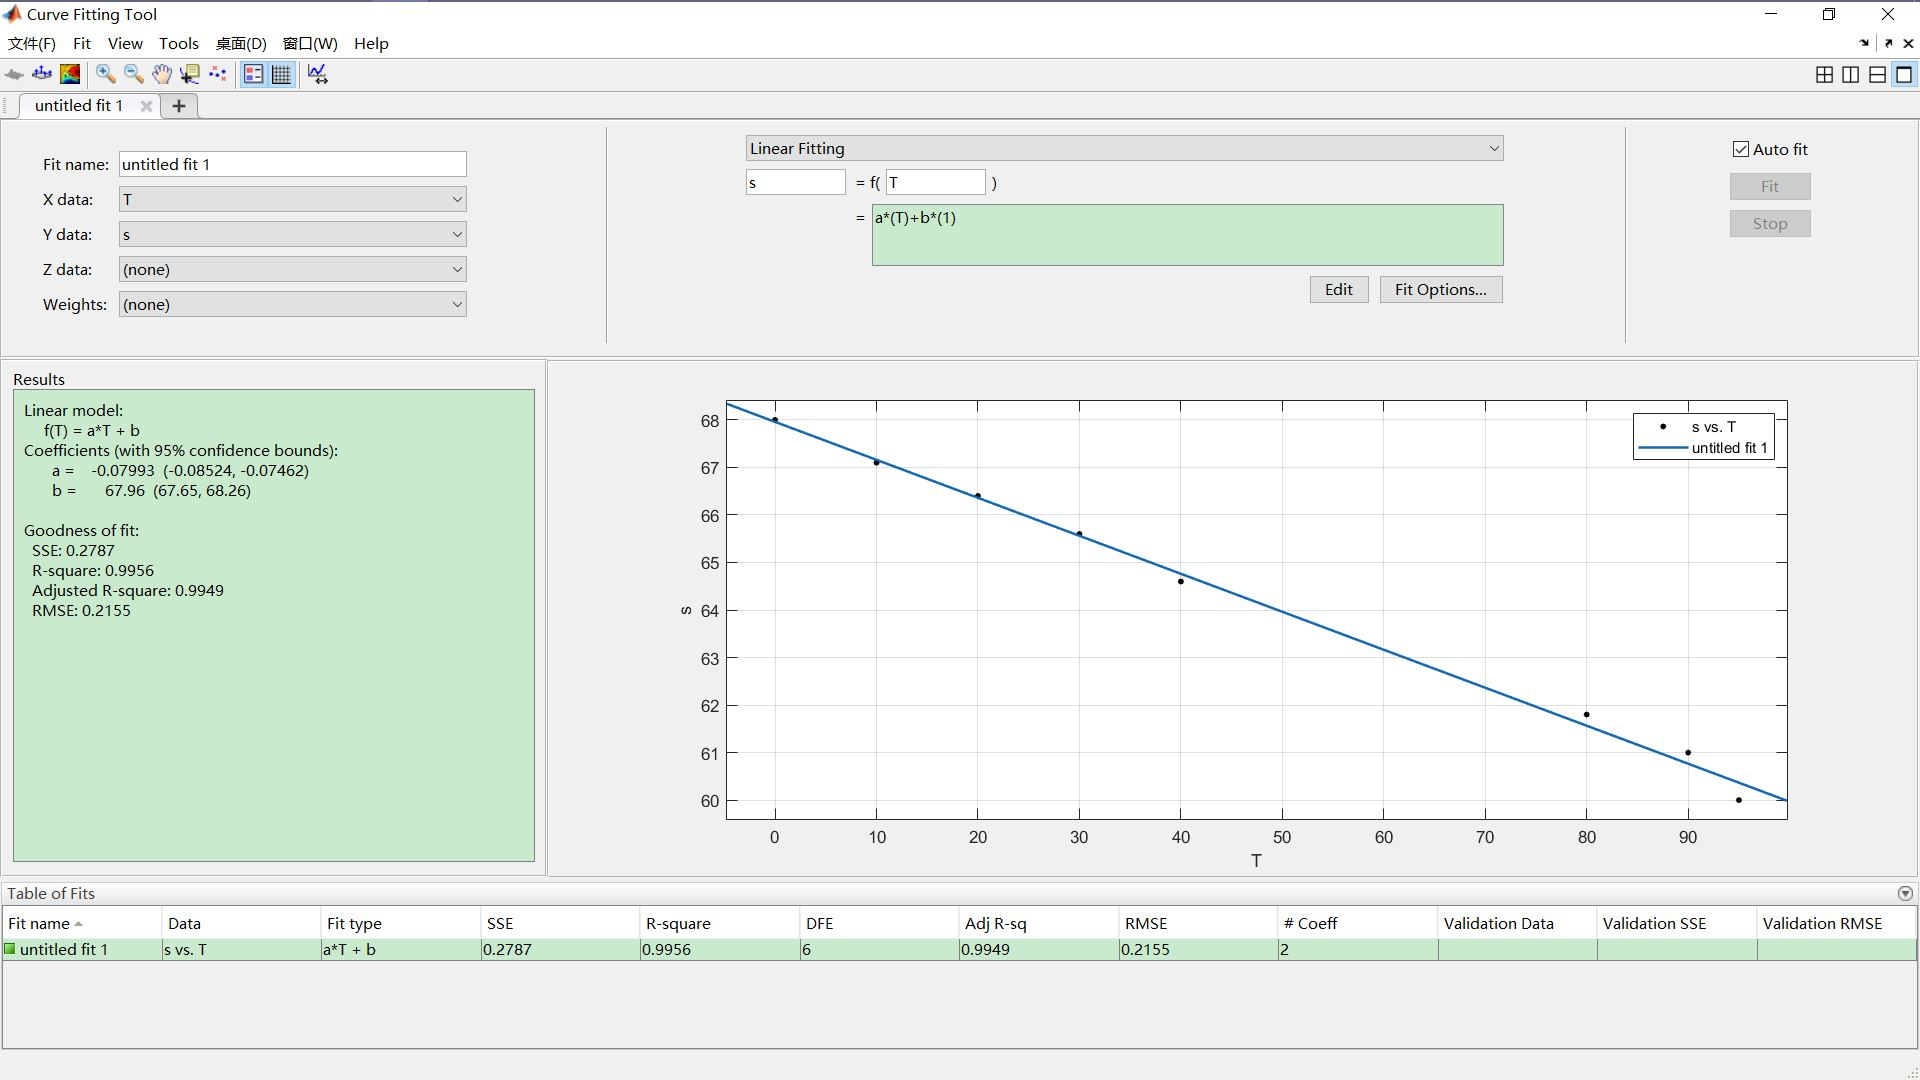
\includegraphics[scale=0.32]{tension.jpg}
            \caption{表面张力--温度拟合}
        \end{figure}
        可见$a = -0.07993$, $b = 67.96$.
    \end{solution}

    \begin{problem}
        拟合形如$f(x) \approx \sfrac{(a+bx)}{(1+cx)}$的函数的一种快速方法是将
        最小二乘法用于如下问题: $f(x)(1+cx)\approx a+bx$,
        试用这一方法拟合\ref{table_population}给出的中国人口数据.
        \begin{table}[H]
            \begin{center}
                \caption{中国人口数据}
                \label{table_population}
                \begin{tabular}{ccc}
                    \Xhline{1.2pt}
                    次序 & 年份 & 人口(亿)\\
                    \hline
                    第一次 & 1953 & 5.82\\
                    第二次 & 1964 & 6.95\\
                    第三次 & 1982 & 10.08\\
                    第四次 & 1990 & 11.34\\
                    第五次 & 2000 & 12.66\\
                    \Xhline{1.2pt}
                \end{tabular}
            \end{center}
        \end{table}
    \end{problem}

    \begin{solution}
        用cftool.
        \begin{figure}[H]
            \centering
            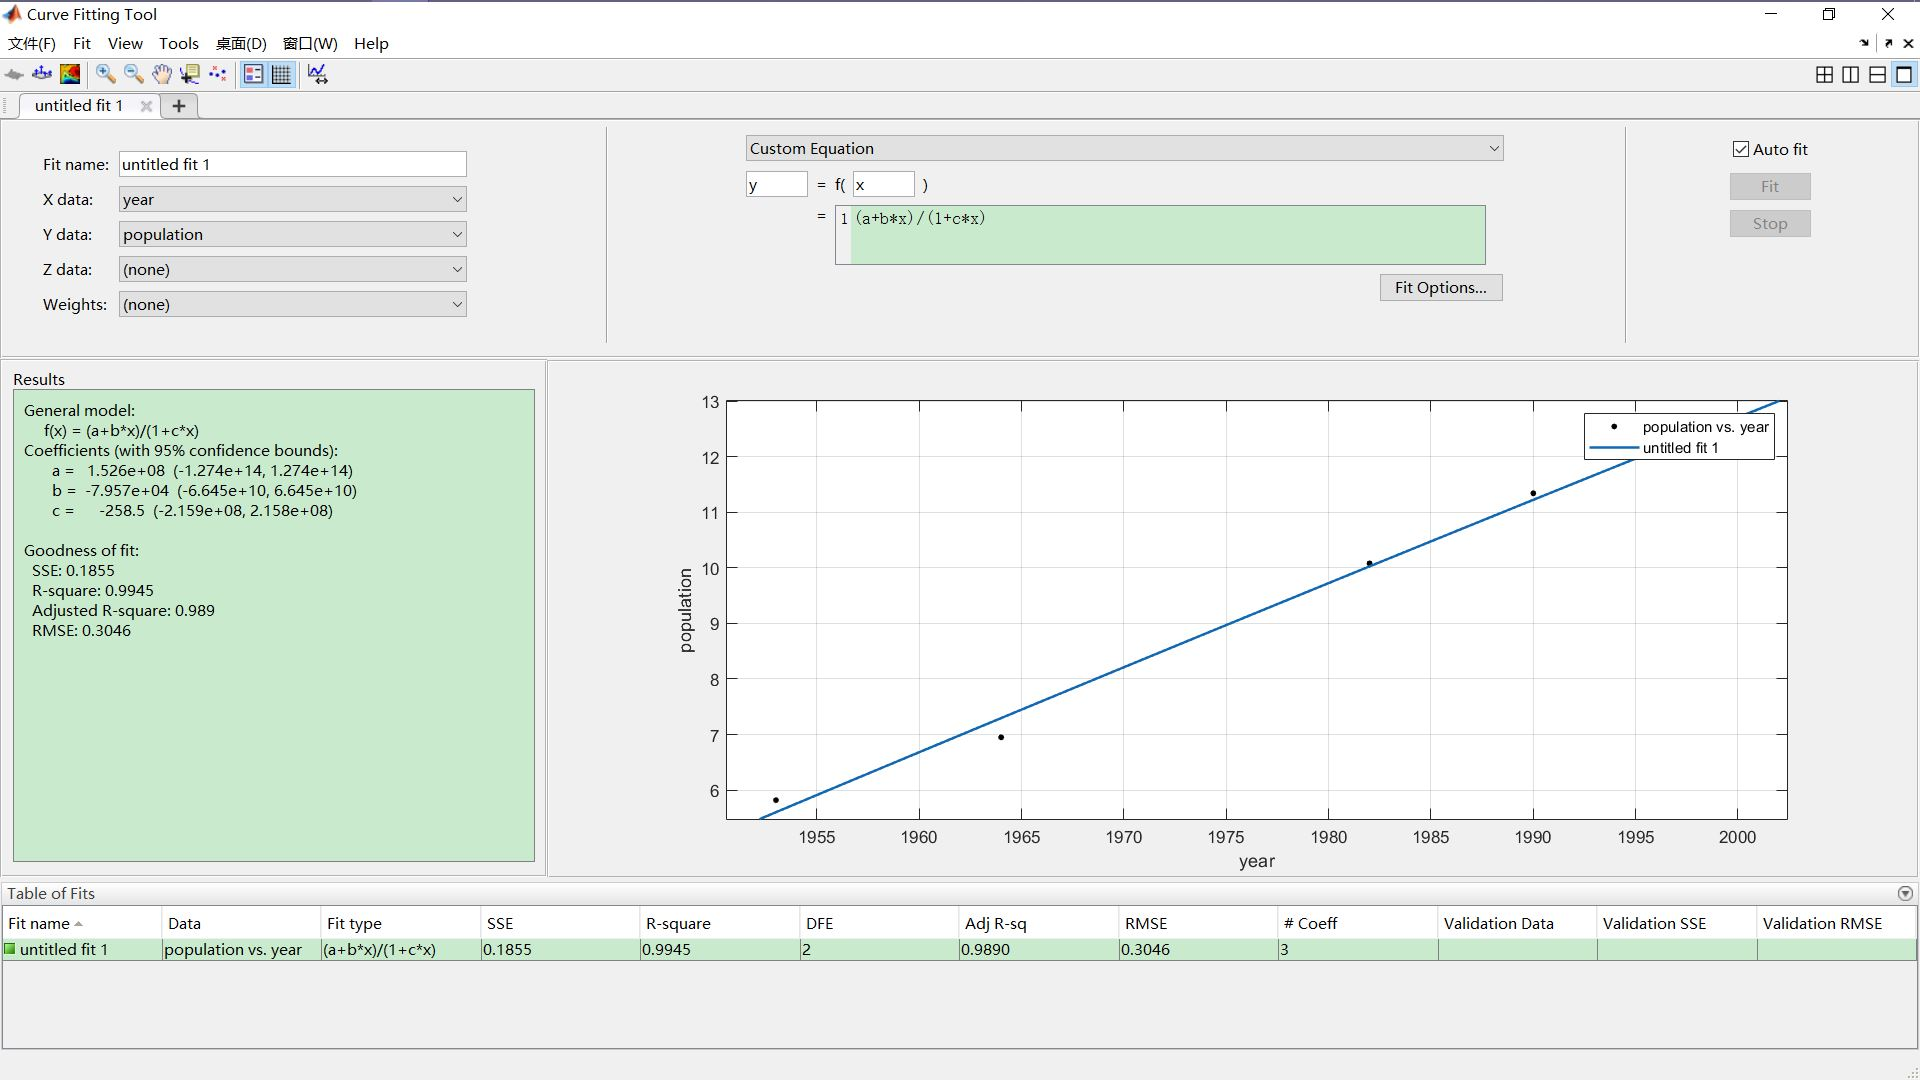
\includegraphics[scale=0.32]{population.jpg}
            \caption{中国人口拟合}
        \end{figure}
        即得出$a$,$b$和$c$的值.
    \end{solution}

    % -------------------- Bibliography --------------------

    % \newpage
    % \bibliography{Principles_of_Mathematical_Analysis}
    % \bibliographystyle{plain}

\end{document}
